
\section{Introduction}

\citet{Ronquist2012a} 

Exercise is in Section \ref{sect:RB-ExerciseMain}.

\subsection{Models}

\subsubsection{Sequence Evolution}

Point to other tutorials (e.g., GTR stuff) 

\subsubsection{Morphological Character Change}

Mk models and ascertainment bias

\subsubsection{Lineage-Specific Substitution Rates}

Clocks \citep{Zuckerkandl1962} and relaxing them 

\subsubsection{Lineage Diversification and Sampling}

Birth-death processes and FBD

\section{Prerequisites}

What do you need to know before doing this?

\subsection{Requirements}
We assume that you have read and hopefully completed the following tutorials:
\begin{itemize}
\item RB\_Getting\_Started
\item RB\_Basics\_Tutorial
\end{itemize}
Note that the RB\_Basics\_Tutorial introduces the basic syntax of \Rev but does not cover any phylogenetic models.
You may skip the RB\_Basics\_Tutorial if you have some familiarity with \R.
We tried to keep this tutorial very basic and introduce all the language concepts on the way.
You may only need the RB\_Basics\_Tutorial for a more in-depth discussion of concepts in \Rev.




\section{Exercise: Estimating the Phylogeny and Divergence Times of Fossil and Extant Bears}\label{sect:RB-ExerciseMain}

Information about the exercise, citations for the data, questions. 

%TODO Background
%%%%%%%%
%%   Data   %%
%%%%%%%%
\subsection{Data files}\label{subsect:RB-DataFiles}

We provide the data files which we will use in this tutorial.
You may want to use your own data instead.
In the \cl{data} folder, you will find the following files
\begin{itemize}[noitemsep,topsep=0pt]
\item \cl{bears\_taxa.tsv}: a list of every taxon in this analysis
\item \cl{bears\_cytb.nex}: an alignment in NEXUS format of 1,000 bp of cytochrome-b sequences for 10 bear species. This alignment includes 8 living bears and 2 extinct sub-fossil bears.
\item \cl{bears\_morphology.nex}: 
\item \cl{bears\_fossil\_intervals.tsv}:
\end{itemize}


\bigskip
\subsection{Getting Started}\label{subsect:RB-GetStart}

{\begin{framed}
On your own computer, create a directory called {\textcolor{red}{\cl{RB\_TotalEvidenceDating\_FBD\_Tutorial}}} (or any name you like). 

In this directory download and unzip the archive containing the data files: \href{www.revbayes.com}{\cl{data.zip}}.

Additionally, create a new directory (in \cl{RB\_TotalEvidenceDating\_FBD\_Tutorial}) called {\textcolor{red}{\cl{scripts}}}
\end{framed}}

When you execute \RevBayes in this exercise, you will do so within the main directory you created (\cl{RB\_TotalEvidenceDating\_FBD\_Tutorial}).

%TODO Stuff about how to start or Rev basics?

%We will complete this analysis in \RevBayes by entering the \Rev code interactively. 
%
%Note that some PDF viewers render some characters differently and if you copy/paste directly from this document, you may introduce erroneous characters. 
%This can cause commands to fail. 
%For learning, it's often better to `live code' and type the commands in manually, rather than copying and pasting. 
%
%Hints for navigating in the \RevBayes console:
%\begin{itemize}[noitemsep,topsep=0pt]
%    \item \cl{Ctrl+A} -- jump to the beginning of the line
%    \item \cl{Ctrl+E} -- jump to the end of the line
%    \item Pressing the up key will pull up previous commands, and allow you to edit them
%    \item If you enter the first few letters of a \RevBayes keyword and then the \textsc{Tab} key, this will `autocomplete' the remaining letters.
%    \item Help -- if you type \cl{?} followed immediately by a \RevBayes keyword, this will print the help pages for that keyword to the screen. (Example \cl{?dnBDP})
%\end{itemize}
%%In \RevBayes, \cl{Ctrl+A} allows you to jump to the start of the command, if you need to delete extra characters from the front of a line. \cl{Ctrl+E} allows you to jump to the end of a command. Pressing the up key will pull up previous commands, and allow you to edit them. If you do choose to copy and paste in commands, doing that from the tutorial script file will cause fewer errors. 

\bigskip

\subsection{Creating \Rev Files}\label{subsect:RB-CreatingFiles}

For complex models and analyses, it is best to create \Rev script files that will contain all of the model parameters, moves, and functions. 
In this exercise, you will work primarily in your text editor and create a set of modular files that will be easily managed and interchanged.
You will write the following files from scratch and save them in the \cl{scripts} directory:
\begin{itemize}[noitemsep,topsep=0pt]
\item \cl{mcmc\_TEFBD.Rev}: the master \Rev file that loads the data, the separate model files, and specifies the monitors and MCMC sampler.
\item \cl{model\_FBDP\_TEFBD.Rev}: specifies the model parameters and moves required for the fossilized birth-death prior on the tree topology, divergence times, fossil occurrence times, and diversification dynamics.
\item \cl{model\_UCExp\_TEFBD.Rev}: specifies the components of the uncorrelated exponential model of lineage-specific substitution rate variation.
\item \cl{model\_GTRG\_TEFBD.Rev}: specifies the parameters and moves for the general-time reversible model of sequence evolution with gamma-distributed rates across sites (GTR+$\Gamma$).
\item \cl{model\_Morph\_TEFBD.Rev}: specifies the model describing discrete morphological character change (binary characters) under a strict morphological clock. 
\end{itemize}

All of the files that you will create are also provided in the \RevBayes tutorial repository. 
Please refer to these files to verify or troubleshoot your own scripts. 
%TODO add link to scripts

\bigskip
\subsection{Start the Master \Rev File and Import Data}\label{subsect:RB-StartMasterRev}



{\begin{framed}
Open your text editor and create the master \Rev file called {\textcolor{red}{\cl{mcmc\_TEFBD.Rev}}} in the \cl{scripts} directory.

Enter the \Rev code provided in this section in the new model file.
\end{framed}}

\medskip
\subsubsection{Load Taxon List}\label{subsub:RB-TaxList}

Now we read in the full list of taxa and create a workspace object with the total number of taxa. 

{\tt \begin{snugshade*}
\begin{lstlisting}
taxa <- readTaxonData("data/bears_taxa.tsv", delimiter=TAB)
n_taxa <- taxa.size() # the number of taxa
\end{lstlisting}
\end{snugshade*}}

\medskip
\subsubsection{Load Data Matrices}\label{subsub:RB-LoadData}

\RevBayes uses the function \cl{readDiscreteCharacterData()} to load a data matrix to the workspace from a formatted file. 
This function can be used for both molecular sequences and discrete morphological characters.

Load the cytochrome-b sequences from file and assign the data matrix to a variable called \cl{cytb}.
{\tt \begin{snugshade*}
\begin{lstlisting}
cytb <- readDiscreteCharacterData("data/bears_cytb.nex") 
\end{lstlisting}
\end{snugshade*}}
%Executing these lines initializes the data matrix as the respective \Rev variables. 
%To report the current value of any variable, simply type the variable name and press enter. For the \cl{cytb} data matrix, this provides information about the alignment:
%{\tt \begin{snugshade*}
%\begin{lstlisting}
%cytb
%|*      DNA character matrix with 10 taxa and 1000 characters
%|*   =====================================================
%|*   Origination:                      bears_cytb.nex
%|*   Number of taxa:                   10
%|*   Number of included taxa:          10
%|*   Number of characters:             1000
%|*   Number of included characters: 1000
%|*   Datatype:                         DNA
%\end{lstlisting}
%\end{snugshade*}}

Next, import the morphological character matrix and assign it to the variable \cl{morpho}. 
{\tt \begin{snugshade*}
\begin{lstlisting}
morpho <- readDiscreteCharacterData("data/bears_morphology.nex")
\end{lstlisting}
\end{snugshade*}}

%The information about the morphological character matrix should look like this:
%
%{\tt \begin{snugshade*}
%\begin{lstlisting}
%morpho
%|*    Standard character matrix with 18 taxa and 81 characters
%|*    ========================================================
%|*    Origination:                   bears_morphology.nex
%|*    Number of taxa:                18
%|*    Number of included taxa:       18
%|*    Number of characters:          81
%|*    Number of included characters: 81
%|*    Datatype:                      Standard
%\end{lstlisting}
%\end{snugshade*}}


If you open the bears taxa file (\cl{bears\_taxa.tsv}), you'll notice that this is a tab-separated file of all of the taxon names, with the age in millions of years ago (mya) in the second column. 
An age of 0.0 indicates an extant bear species. 
We will use this information to allow fossils to be incorporated as tips in the analysis. 

\medskip
\subsubsection{Add Missing Taxa}\label{subsub:RB-AddMissing}

Notice that the two data matrices have different numbers of taxa. The last bit of data preparation we will do is to add any taxa that are not found in the molecular partition (i.e. are only found in the fossil data) to the molecular partition as missing data, and vice versa.
In order for all the taxa to appear on the same tree, they all need to be part of the same dataset, as opposed to present in separate datasets. 
This ensures that there is a unified taxon set that contains all of our tips.

{\tt \begin{snugshade*}
\begin{lstlisting}
cytb.addMissingTaxa( taxa )
morpho.addMissingTaxa( taxa )
\end{lstlisting}
\end{snugshade*}}

%
%\bigskip
%
%\subsection{Specify Clades}
%
%RevBayes allows researchers to use clade constraints to put a zero probability on trees not containing certain clades. In our case, Ursinae (brown bears, black bears and sloth bears) and Ailuropodinae (pandas and their close relatives) are both very well supported subfamilies. We will add constraints for these two groups. 
%
%{\tt \begin{snugshade*}
%\begin{lstlisting}
%clade_ursinae = clade("Melursus_ursinus","Ursus_arctos","Ursus_maritimus", 
%                         "Helarctos_malayanus","Ursus_americanus","Ursus_thibetanus", 
%                         "Ursus_abstrusus","Ursus_spelaeus")
%clade_pandas = clade("Ailuropoda_melanoleuca","Indarctos_vireti",
%                        "Indarctos_arctoides","Indarctos_punjabiensis", 
%                        "Ailurarctos_lufengensis","Agriarctos_spp",
%                        "Kretzoiarctos_beatrix")
%constraints = v(clade_pandas, clade_ursinae)
%\end{lstlisting}
%\end{snugshade*}}
%
%We will also define a clade for the extant bears that will not be constrained. This will allow us to monitor the age of this node in our log file (in Section \ref{?}).
%{\tt \begin{snugshade*}
%\begin{lstlisting}
%clade_extant = clade("Ailuropoda_melanoleuca","Tremarctos_ornatus","Melursus_ursinus",
%                       "Ursus_arctos","Ursus_maritimus","Helarctos_malayanus",
%                       "Ursus_americanus","Ursus_thibetanus")
%\end{lstlisting}
%\end{snugshade*}}
%
%\bigskip
%
%\subsection{Create a Helper Variable}

\medskip
\subsubsection{The Move-List Iterator Variable}\label{subsub:RB-mviVar}



%Now that our data are loaded and prepared, we can specify the fossilized birth-death model, and the MCMC moves associated with it. 
%As we work, we will be creating moves to govern how values are sampled for our various priors and parameters. We'll first create an iterator to hold all of our moves.

{\tt \begin{snugshade*}
\begin{lstlisting}
mvi = 1
\end{lstlisting}
\end{snugshade*}}

\bigskip

\subsection{The Fossilized Birth-Death Process}\label{subsect:RB-ModelFBD}

{\begin{framed}
Open your text editor and create the fossilized birth-death model file called {\textcolor{red}{\cl{model\_FBDP\_TEFBD.Rev}}} in the \cl{scripts} directory.

Enter the \Rev code provided in this section in the new model file.
\end{framed}}

Two key parameters of the FBD process are the birth rate (the rate at which lineages are added to the tree) and the death rate (the rate at which lineages are removed from the tree). 
We'll place exponential priors on both of these values. 
An exponential prior with a $\lambda$ =  10 places a higher probability on values closer to zero than one for these parameters. 

{\tt \begin{snugshade*}
\begin{lstlisting}
birth_rate ~ dnExponential(10)
death_rate ~ dnExponential(10)
\end{lstlisting}
\end{snugshade*}}

Now that the priors have been specified, we give RevBayes some information on how to sample values for our parameters. 
We'll use a scaling move, which changes the value sampled multiplicatively with the tuning parameter. 
We will use three different tuning parameters, which govern the size of the move. 
Including multiple tuning parameters improves mixing. 

{\tt \begin{snugshade*}
\begin{lstlisting}
moves[mvi++] = mvScale(birth_rate, lambda=0.01, weight=3.0)
moves[mvi++] = mvScale(birth_rate, lambda=0.1, weight=3.0)
moves[mvi++] = mvScale(birth_rate, lambda=1.0, weight=3.0)
moves[mvi++] = mvScale(death_rate, delta=0.01, weight=3.0)
moves[mvi++] = mvScale(death_rate, delta=0.1, weight=3.0)
moves[mvi++] = mvScale(death_rate, delta=1, weight=3.0)
\end{lstlisting}
\end{snugshade*}}

In order to print the states of model variables output files (also called \textit{monitoring}), we need to create deterministic nodes for the diversification and turnover. 
Deterministic nodes are value transformations between existing stochastic nodes. 
So we will define diversification and turnover as deterministic nodes.

{\tt \begin{snugshade*}
\begin{lstlisting}
diversification := birth_rate - death_rate
turnover := death_rate/birth_rate
\end{lstlisting}
\end{snugshade*}}

All extant bears are represented in this dataset. 
Therefore, we can fix the sampling probability of extant lineages to 1.

{\tt \begin{snugshade*}
\begin{lstlisting}
rho <- 1.0
\end{lstlisting}
\end{snugshade*}}

The rate of sampling fossils ($\psi$), on the other hand is not known. 
We will use an exponential prior on this parameter as well, and use a slide move to sample values from our distribution.

{\tt \begin{snugshade*}
\begin{lstlisting}
psi ~ dnExponential(10) 
moves[mvi++] = mvScale(birth_rate, lambda=0.01, weight=3.0)
moves[mvi++] = mvScale(birth_rate, lambda=0.1, weight=3.0)
moves[mvi++] = mvScale(birth_rate, lambda=1.0, weight=3.0)
\end{lstlisting}
\end{snugshade*}}

Under the FBD model, the process is conditioned on the age of the origin, or the start of the process. 
We will specify a uniform distribution on the age of the origin. If you looked in the bears taxa file, you might notice that the age of the oldest fossil is slightly younger than the upper bound of the uniform distribution on the origin age. 
For this parameter, we will use a sliding window move. A sliding window move samples within an interval (defined by \cl{delta}). 
Sliding window moves can be tricky for small values, as the window may overlap zero. 
However, for parameters such as the origin, there is little risk of this being an issue.

{\tt \begin{snugshade*}
\begin{lstlisting}
origin_time ~ dnUnif(37.0, 55.0)
moves[mvi++] = mvSlide(origin_time, delta=0.01, weight=10.0)
moves[mvi++] = mvSlide(origin_time, delta=0.1, weight=10.0)
moves[mvi++] = mvSlide(origin_time, delta=1, weight=10.0)
\end{lstlisting}
\end{snugshade*}}

All the parameters of the FBD process are now defined. 
The next step is to combine these parameters to define the tree prior as the FBD.

{\tt \begin{snugshade*}
\begin{lstlisting}
tree_prior = dnFBDP(origin=origin_time, lambda=birth_rate, mu=death_rate, psi=psi, rho=rho, taxa=taxa)
\end{lstlisting}
\end{snugshade*}}

Next, we will define the \cl{fbd\_tree} variable as a random variable. 
It will be used to generate trees under the FBD process that conform to our clade constraints. 

{\tt \begin{snugshade*}
\begin{lstlisting}
fbd_tree ~ dnConstrainedTopology(tree_prior, constraints) 
\end{lstlisting}
\end{snugshade*}}

Finally, we can also create deterministic nodes for other quantities we might be interested in monitoring. 
Below, we will define a monitor that prints the number of fossils that are inferred to be `sampled ancestors' - lineages that are present in the phylogeny, and have descendants present on the tree. 
We will also define a deterministic node for the age of the crown group of bears, using the previously-defined extant bear constraint (Section \ref{}).

{\tt \begin{snugshade*}
\begin{lstlisting}
sa := fbd_tree.numSampledAncestors();
crown := tmrca(fbd_tree, clade_extant)
\end{lstlisting}
\end{snugshade*}}

\bigskip

\subsection{The Uncorrelated Exponential Relaxed-Clock Model}\label{subsect:RB-ModelUCExp}

{\begin{framed}
Open your text editor and create the lineage-specific branch-rate model file called {\textcolor{red}{\cl{model\_UCExp\_TEFBD.Rev}}} in the \cl{scripts} directory.

Enter the \Rev code provided in this section in the new model file.
\end{framed}}


\bigskip

\subsection{The General-Time Reversible Gamma-Rates Model of Sequence Evolution}\label{subsect:RB-ModelGTRG}

{\begin{framed}
Open your text editor and create the molecular substitution model file called {\textcolor{red}{\cl{model\_GTRG\_TEFBD.Rev}}} in the \cl{scripts} directory.

Enter the \Rev code provided in this section in the new model file.
\end{framed}}

\bigskip

\subsection{Modeling the Evolution of Binary Morphological Characters}\label{subsect:RB-ModelMorph}

{\begin{framed}
Open your text editor and create the morphological character model file called {\textcolor{red}{\cl{model\_Morph\_TEFBD.Rev}}} in the \cl{scripts} directory.

Enter the \Rev code provided in this section in the new model file.
\end{framed}}

Morphology has traditionally been assumed to evolve according to a generalized Jukes-Cantor matrix in which all characters have the same transition rates, and all characters have an equal probability of making forwards or backwards transitions (i.e., the same probability of going from 0 to 1 as 1 to 0). 
This model is called the Mk model. We will use a hyperprior on state frequencies to relax these two assumptions. 
Because we are working with binary data, we can use a discrete Beta distribution to describe the variation in stationary state frequencies across characters. 
The Beta distribution has two parameters, $\alpha$ and $\beta$ which describe its shape. 
For simplicity, we will assume that $\alpha$ = $\beta$. 
The below code draws a value for $\beta$ from an exponential distribution and places a move on it.

{\tt \begin{snugshade*}
\begin{lstlisting}
beta_hp ~ dnExponential( 1.0 )

moves[mvi++] = mvScale(beta_hp, lambda=1,    weight=1.0 )
moves[mvi++] = mvScale(beta_hp, lambda=0.1,  weight=1.0 )
moves[mvi++] = mvScale(beta_hp, lambda=0.01, weight=1.0 )
\end{lstlisting}
\end{snugshade*}}

Next, we'll create a vector containing four different site stationary state frequencies. 
This is similar to allowing gamma-distributed rate variation across sites. 
We will then use these stationary frequencies to generate a set of new Q-matrices which do not enforce the assumptions of the same transition rates at every site and equal forward and backwards transition rates.

{\tt \begin{snugshade*}
\begin{lstlisting}
beta_cats := fnDiscretizeBeta( beta_hp, beta_hp, 4)
for(i in 1:beta_cats.size())
{
    Q_morpho[i] := fnFreeBinary(v(1-beta_cats[i], beta_cats[i]))
}
\end{lstlisting}
\end{snugshade*}}


As in the molecular data partition, we will allow gamma-dstributed rate heterogeneity among sites.
{\tt \begin{snugshade*}
\begin{lstlisting}
alpha_morpho ~ dnExponential( 1.0 )
rates_morpho := fnDiscretizeGamma( alpha_morpho, alpha_morpho, 4, false )

moves[mvi++] = mvScale(alpha_morpho, lambda=0.01, weight=1.0)
moves[mvi++] = mvScale(alpha_morpho, lambda=0.1,  weight=1.0)
moves[mvi++] = mvScale(alpha_morpho, lambda=1,    weight=1.0)
\end{lstlisting}
\end{snugshade*}}

Each data partition has to have a clock rate. For simplicity, we will assume a strict clock rate drawn from an exponential distribution.

{\tt \begin{snugshade*}
\begin{lstlisting}
clock_morpho ~ dnExponential(1.0)

moves[mvi++] = mvScale(clock_morpho, lambda=0.01, weight=4.0)
moves[mvi++] = mvScale(clock_morpho, lambda=0.1,  weight=4.0)
moves[mvi++] = mvScale(clock_morpho, lambda=1,    weight=4.0)
\end{lstlisting}
\end{snugshade*}}

As in our molecular data partition, we now combine our data and our model. There are some unique aspects to doing this for morphology. \par
You will notice that we have a variable called `coding'. This variable allows us to condition on biases in the way the morphological data were collected.
Morphology is often collected to maximize the amount of variation present in the dataset. 
This has traditionally been accomplished by collecting characters that exhibit parsimony informativity (i.e., those that can be used under the parsimony optimality criterion to discriminate among tree hypotheses) in the group of interest, or those that exhibit any variation in the group of interest. 
This means few datasets contain invariant characters. 
The lack of invariant characters can bias estimates of branch lengths towards unrealistically long lengths.
Therefore, we specify a correction to account for the fact that invariant sites have no been observed.
In the case of this dataset, parsimony non-informative variable characters, such as autapomorphies, have been collected. 
We will, therefore, use the `variable' correction to account for this. \par

We use the flag `siteMatrices=true' to indicate that we are providing multiple Q matrices generated as a function of our state frequency variation model. \par


{\tt \begin{snugshade*}
\begin{lstlisting}
phyMorpho ~ dnPhyloCTMC(tree=fbd_tree, siteRates=rates_morpho, branchRates=clock_morpho, Q=Q_morpho, type="Standard", coding="variable", siteMatrices=true)
phyMorpho.clamp(morpho)
\end{lstlisting}
\end{snugshade*}}


\bigskip

\subsection{Complete MCMC File}\label{subsect:RB-CompleteMCMC}

{\begin{framed}
Return to the master \Rev file you created in Section \ref{subsect:RB-StartMasterRev} called {\textcolor{red}{\cl{mcmc\_TEFBD.Rev}}} in the \cl{scripts} directory.

Enter the \Rev code provided in this section in this file.
\end{framed}}

\medskip
\subsubsection{Source Model Scripts}\label{subsub:RB-SourceMods}
{\tt \begin{snugshade*}
\begin{lstlisting}
source("scripts/model_FBDP_TEFBD.Rev")

source("scripts/model_UCExp_TEFBD.Rev")

source("scripts/model_GTRG_TEFBD.Rev")

source("scripts/model_Morph_TEFBD.Rev")
\end{lstlisting}
\end{snugshade*}}



\medskip
\subsubsection{Create Model Object}\label{subsub:RB-ModObj}


{\tt \begin{snugshade*}
\begin{lstlisting}
mymodel = model(sf)
\end{lstlisting}
\end{snugshade*}}

\medskip
\subsubsection{Specify Monitors and Output Filenames}\label{subsub:RB-Monitors}


{\tt \begin{snugshade*}
\begin{lstlisting}
mni = 1
monitors[mni++] = mnModel(filename="output/bears.log", printgen=10)
monitors[mni++] = mnFile(filename="output/bears.trees", printgen=10, fbd_tree)
monitors[mni++] = mnScreen(printgen=10, age_extant, num_samp_anc, origin_time)
\end{lstlisting}
\end{snugshade*}}

\medskip
\subsubsection{Set up the MCMC}


{\tt \begin{snugshade*}
\begin{lstlisting}
mymcmc = mcmc(mymodel, monitors, moves)

mymcmc.run(generations=10000)
\end{lstlisting}
\end{snugshade*}}

{\begin{framed}
Save and close all files.
\end{framed}}

\bigskip
\subsection{Run it}\label{subsect:RB-RunMCMC}


{\tt \begin{snugshade*}
\begin{lstlisting}
./rb
\end{lstlisting}
\end{snugshade*}}

Execute the MCMC analysis:
{\tt \begin{snugshade*}
\begin{lstlisting}
source("scripts/mcmc_TEFBD.Rev")
\end{lstlisting}
\end{snugshade*}}

{\tiny{\tt \begin{snugshade*}
\begin{lstlisting}
|*   Processing file "scripts/mcmc_TEFBD.Rev"
|*   Successfully read one character matrix from file 'data/bears_cytb.nex'
|*   Successfully read one character matrix from file 'data/bears_morphology.nex'
|*   Processing file "scripts/model_FBDP_TEFBD.Rev"
|*   Processing of file "scripts/model_FBDP_TEFBD.Rev" completed
|*   Processing file "scripts/model_UCExp_TEFBD.Rev"
|*   Processing of file "scripts/model_UCExp_TEFBD.Rev" completed
|*   Processing file "scripts/model_GTRG_TEFBD.Rev"
|*   Processing of file "scripts/model_GTRG_TEFBD.Rev" completed
|*   Processing file "scripts/model_Morph_TEFBD.Rev"
|*   Processing of file "scripts/model_Morph_TEFBD.Rev" completed
|*
|*   Running MCMC simulation
|*   This simulation runs 1 independent replicate.
|*   The simulator uses 163 different moves in a random move schedule with 267 moves per iteration
|*
|*Iter        |      Posterior   |     Likelihood   |          Prior   |     age_extant   |   num_samp_anc   |    origin_time   |    elapsed   |        ETA   |
|*---------------------------------------------------------------------------------------------------------------------------------------------
|*0           |       -8174.01   |        -8053.8   |       -120.209   |        34.8641   |              0   |        44.4332   |   00:00:00   |   --:--:--   |
|*10          |       -4654.95   |        -4611.2   |       -43.7495   |        4.32618   |              7   |        45.4494   |   00:00:01   |   --:--:--   |
|*20          |       -4294.05   |       -4266.91   |       -27.1443   |        4.58804   |              7   |        46.5636   |   00:00:01   |   00:08:19   |
|*30          |       -4267.35   |       -4233.41   |         -33.94   |         6.8467   |              6   |        45.9177   |   00:00:02   |   00:11:04   |
|*40          |       -4226.63   |       -4188.32   |       -38.3037   |        6.40484   |              8   |        44.3696   |   00:00:02   |   00:08:18   |
|*...
\end{lstlisting}
\end{snugshade*}}}

\bigskip
\subsection{Summarize Your Results}\label{subsect:RB-SummarizeResults}

\medskip
\subsubsection{Evaluate MCMC}\label{subsub:RB-EvalMCMC}

%TODO this is tracer stuff


\medskip
\subsubsection{Summarize Tree}\label{subsub:RB-SummarizeTree}

%TODO this they can do interactively in rb

Start up RevBayes at the command line. You should do this from within the \cl{RB\_TotalEvidenceDating\_FBD\_Tutorial} directory.
{\tt \begin{snugshade*}
\begin{lstlisting}
./rb
\end{lstlisting}
\end{snugshade*}}

Read in the MCMC sample of trees from file.
{\tt \begin{snugshade*}
\begin{lstlisting}
trace = readTreeTrace("output/bears.trees")

for(i in 1:trace.size())
{
    trees[i] = fnPruneTree(trace.getTree(i), pruneTaxa=v(taxa[17],taxa[20]))
}

trace_pruned = treeTrace(trees)
mccTree(trace_pruned, "output/bears.mcc.tre" )
\end{lstlisting}
\end{snugshade*}}

See Fig.\ \ref{fig:IcyTreeSumm}

\begin{figure}[h!]
\centering
\fbox{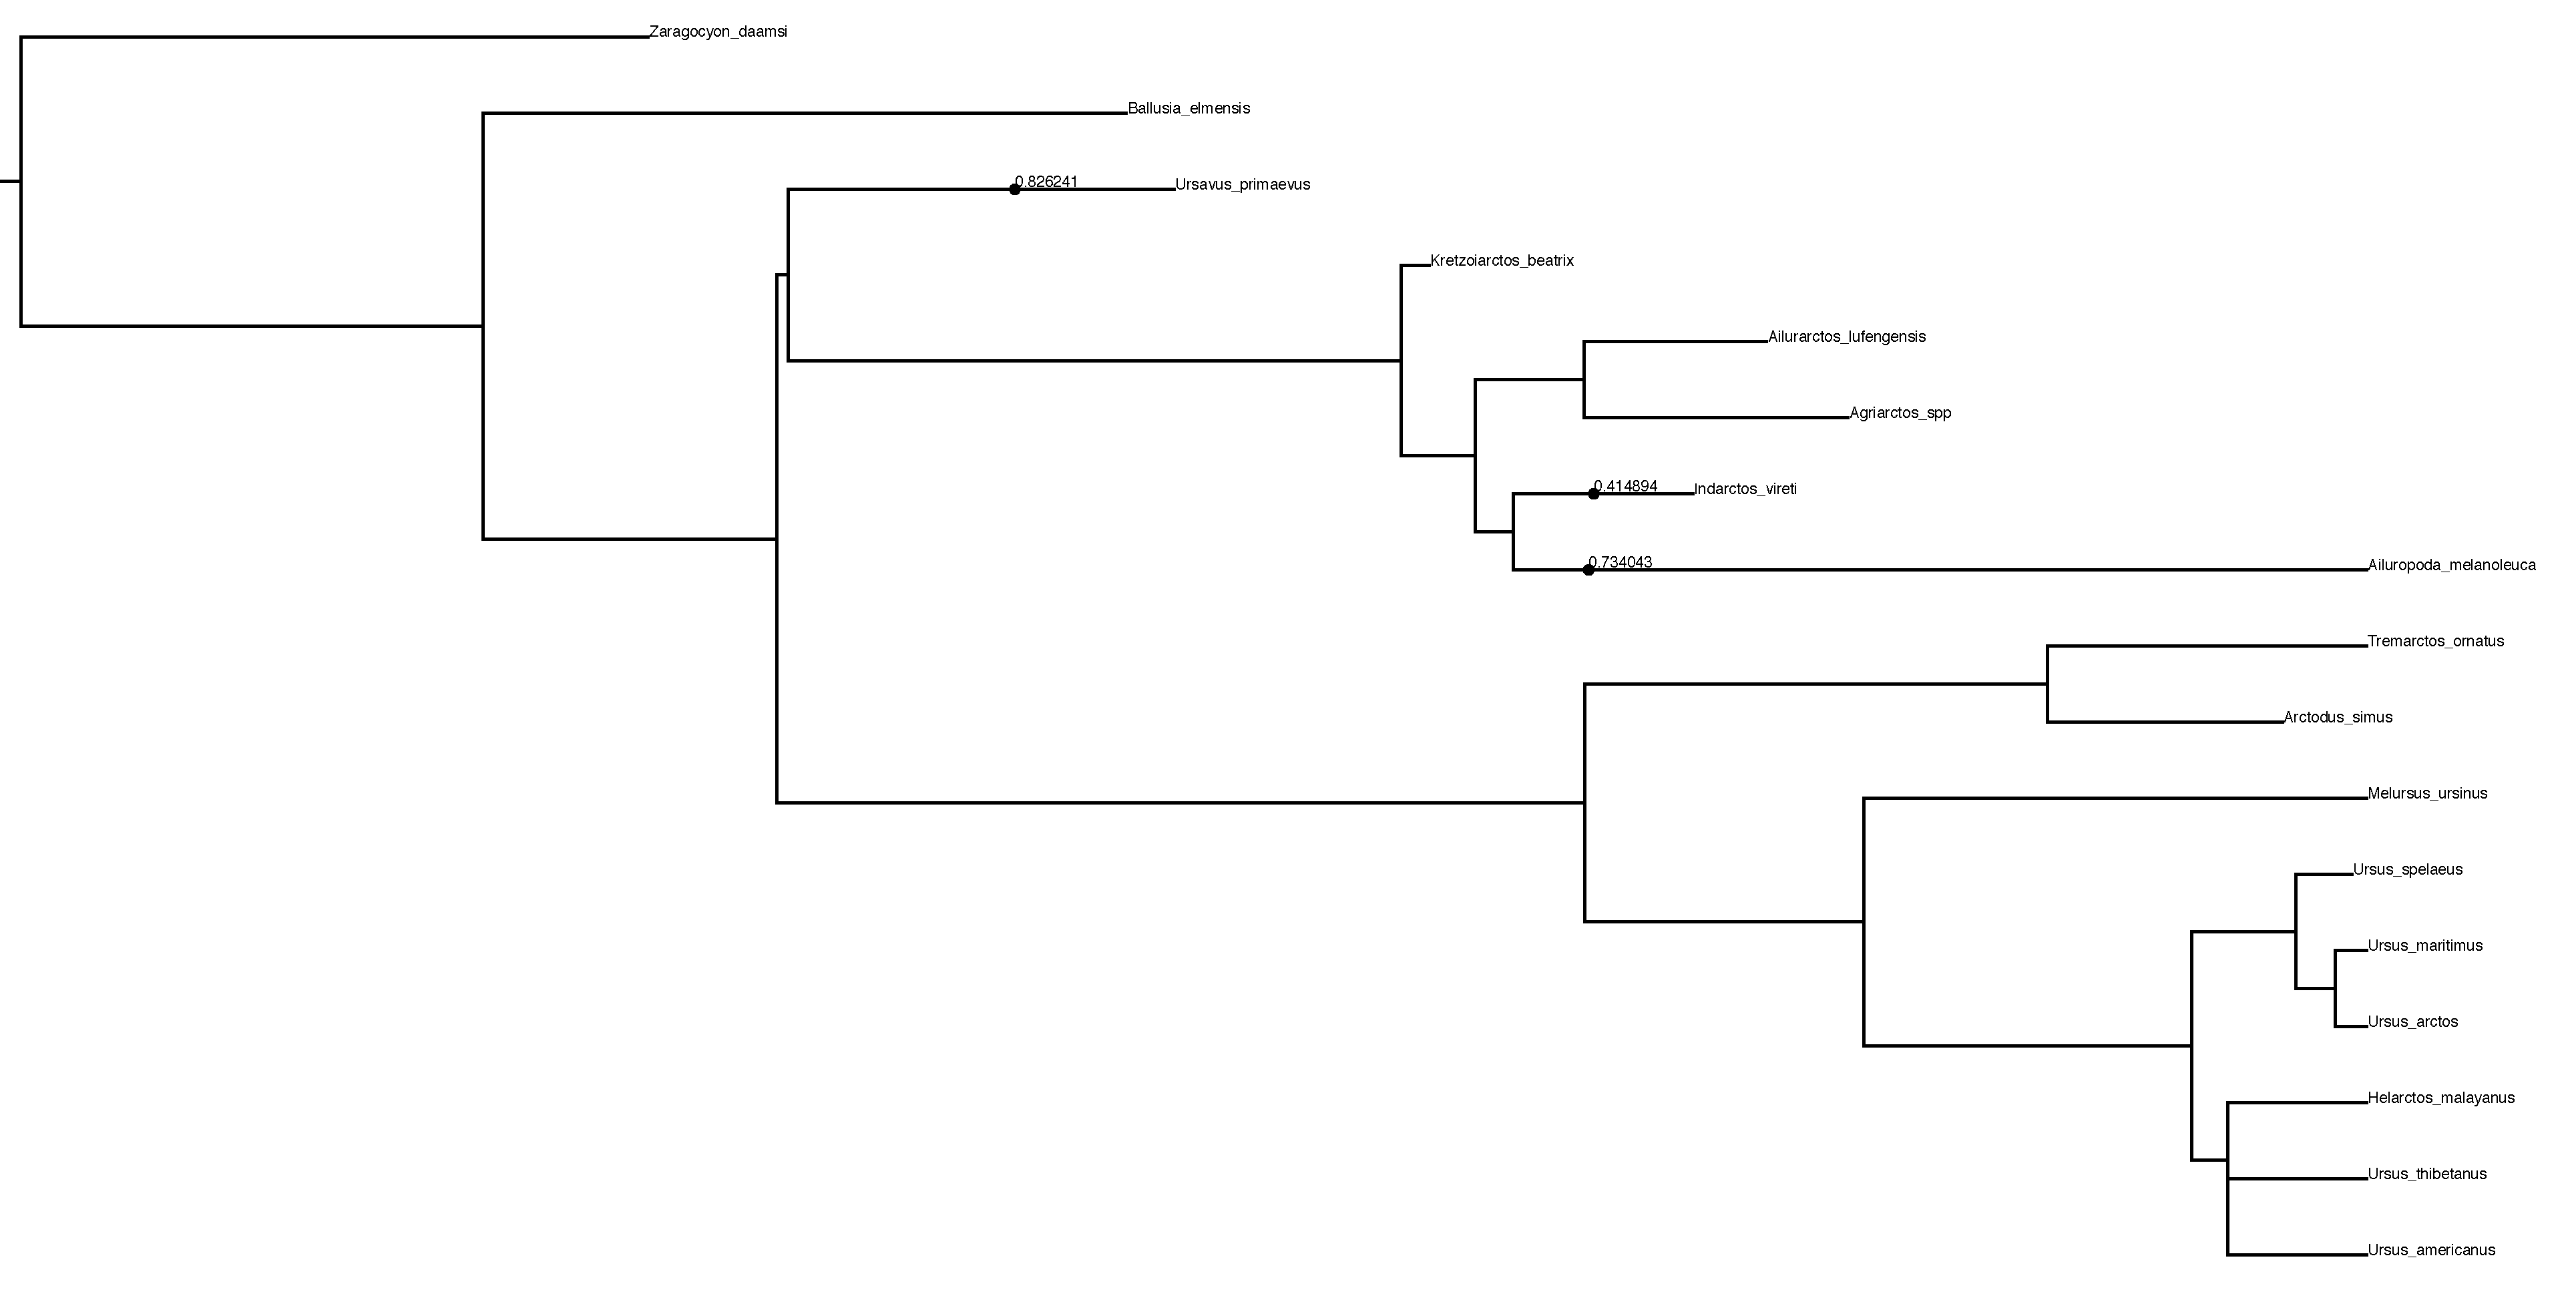
\includegraphics[width=\textwidth,angle=0]{\ResourcePath figures/summary_tree.pdf}}
\caption{\small This is a place-holder figure.}
\label{fig:IcyTreeSumm}
\end{figure}


%TODO IcyTree

\bibliographystyle{sysbio}
\bibliography{\GlobalResourcePath refs}
